\chapter{Supplementary External-Method Comparisons}
\label{chap:external-comparisons}

\section{Scope and evidence}

The internal Swin-T comparison tests the effect of adding the implemented
regional graph to a shared backbone. A complementary question is how that
design compares with complete published graph-based scene-classification
methods. HGTNet~\cite{li2024hgtnet} and DFAGCN~\cite{xu2022dfagcn}, reviewed
in Chapter~\ref{chap:related-work}, provide two relevant architectural
comparators. This chapter reports three completed measurements: HGTNet on
NWPU-RESISC45 and AID, and DFAGCN on NWPU-RESISC45. Each measurement uses
training seed 42. The implementations are independent project versions with
explicit choices where the available method specification was incomplete;
they are not the authors' official implementations or verified reproductions
of the published scores.

The runs reuse the frozen partitions in Table~\ref{tab:partitions}.
NWPU-RESISC45 uses 5,040 calibration-training images, 1,260 validation images,
a 6,300-image final fitting pool and 25,200 test images. AID uses
4,000/1,000/5,000/5,000 images, respectively. Class order and sample identity
are fixed by the original manifests. Validation selects the epoch count
and, for DFAGCN, the linear-classifier parameter. The learned calibration
state is then discarded and final fitting starts afresh on the training
pool. Test predictions are used for final reporting and subsequent error
description, rather than recipe selection.

Original external-method test predictions have been recovered and their
aggregate metrics, class metrics and confusion matrices independently
recomputed locally. The HGTNet calibration and refit histories are also
available. The original AID Swin-T and fixed-GAViT predictions have also
been recovered, matched to all 5,000 ordered test paths and labels, and
recomputed. The internal NWPU reference scores retain their archived
seed42 summaries; the corresponding raw vectors were not recovered in
this analysis. These tables are supplementary single-seed
complete-method comparisons. They neither replace the internal multi-seed
results and component ablations nor complete the required external
multi-seed comparison under a unified training protocol.

\section{Disclosed differences between recipes}

The methods share data partitions, label mappings and the separation of
selection, final fitting and testing. Their backbones, preprocessing,
optimisation and calibration budgets differ. Table~\ref{tab:external-recipes}
summarises the principal differences. Consequently, a score difference
cannot be attributed solely to the presence or type of graph reasoning.

\begin{table}[tbp]
 \centering
 \caption{Principal recipe differences in the supplementary seed42
 comparisons. The common partition does not imply a common training recipe.}
 \label{tab:external-recipes}
 \small
 \setlength{\tabcolsep}{4pt}
 \begin{tabular}{p{0.16\textwidth}p{0.31\textwidth}p{0.43\textwidth}}
  \toprule
  Method & Representation and input & Optimisation and selection\\
  \midrule
  Internal Swin-T / GAViT & Shared pretrained Swin-T;
  RGB resized to $224\times224$. & Batch 32; AdamW,
  $3\times10^{-4}$ learning rate, $10^{-4}$ weight decay;
  30-epoch cosine calibration, followed by fresh refit for the selected
  epoch count.\\[0.5em]
  Independent HGTNet & Partial torchvision Swin-B initialisation;
  resize to $256\times256$, then a $224\times224$ crop. & Batch 16;
  Adam, $10^{-5}$ learning rate, $5\times10^{-5}$ weight decay;
  100 calibration epochs, no scheduler, followed by fresh refit for the
  validation-selected epoch count.\\[0.5em]
  Independent DFAGCN & Frozen torchvision VGG16;
  $224\times224$ fully connected features and $448\times448$
  convolutional features; three graph branches and weighted fusion. &
  Graph-branch Adam training, batch 100, initial learning rate $10^{-3}$;
  100-epoch calibration cap and a factor 0.1 decay every 50 epochs;
  validation-only epoch and LIBLINEAR $C$ selection before fresh refit.\\
  \bottomrule
 \end{tabular}
\end{table}

For HGTNet, training uses a random crop after resizing and a horizontal flip
with probability 0.5; evaluation uses a centre crop. Both paths use
ImageNet channel normalisation. Computation is FP32 without AMP or TF32.
The crop details, optimiser defaults, absence of scheduling and selection
rules are disclosed engineering choices rather than asserted original-paper
defaults. Partial Swin-B initialisation does not establish equivalence to
the original method's pretrained model.

DFAGCN uses a separate staged pipeline, not the end-to-end Swin/GAViT
trainer. VGG16~\cite{simonyan2015vgg} features are frozen, while graph
branches are fitted on the permitted training subset. The independent
implementation uses $7\times7$ adaptive pooling, two 256-wide graph
convolutional layers per branch and explicit readout and fusion choices.
Its torchvision weights and RGB stretch resizing do not establish numerical
equivalence to the original MatConvNet preprocessing. The selected final
classifier uses LIBLINEAR with $C=10$, after an independently initialised
51-epoch graph refit. These disclosed choices remain part of the result's
identity.

\section{Single-seed test measurements}

\subsection{NWPU-RESISC45}

Table~\ref{tab:external-nwpu} reports the complete 25,200-image test results.
The external rows are local reconstructions from returned predictions;
the internal rows retain their archived seed 42 values. All scores refer to
final fitting on the 6,300-image pool rather than calibration validation.

% Exact source: results/external_baselines_nwpu_seed42_20261030.csv.
% HGTNet OA=94.11904761904762; macro-F1=94.10529172930384.
% DFAGCN OA=86.53174603174604; macro-F1=86.45890874660422.
\begin{table}[tbp]
 \centering
 \caption{Supplementary NWPU-RESISC45 comparison at training seed 42.
 Scores are percentages; different complete-method recipes are disclosed in
 Table~\ref{tab:external-recipes}. No single-run standard deviation is assigned.}
 \label{tab:external-nwpu}
 \small
 \setlength{\tabcolsep}{5pt}
 \begin{tabular}{lrrrr}
  \toprule
  Model & OA & Macro-F1 & Correct & Refit epochs\\
  \midrule
  Swin-T & 93.9325 & 93.9091 & 23,671 & 29\\
  GAViT, fixed $4\times4$ & 94.1032 & 94.0899 & 23,714 & 29\\
  GAViT, local soft & 93.8690 & 93.8550 & 23,655 & 28\\
  DFAGCN, independent & 86.5317 & 86.4589 & 21,806 & 51\\
  HGTNet, independent & 94.1190 & 94.1053 & 23,718 & 95\\
  \bottomrule
 \end{tabular}
\end{table}

HGTNet exceeds fixed GAViT by approximately 0.015873 pp OA and 0.015358 pp
macro-F1, corresponding to four additional correct predictions in aggregate.
This is a close single-seed point estimate, rather than evidence of
statistical equivalence or a stable ranking. The aggregate difference of
four does not reveal how many individual errors either method corrects or
introduces; that requires both original prediction vectors.

Fixed GAViT exceeds the independent DFAGCN result by approximately
7.571429 pp OA. This compares a fine-tuned Transformer with a frozen-VGG16,
staged graph-and-linear-classifier pipeline under their disclosed recipes.
It does not isolate a graph operator or establish that the published DFAGCN
method has been reproduced. In contrast, the two returned external
prediction vectors can be paired: HGTNet corrects 2,415 DFAGCN errors and
introduces 503 errors relative to DFAGCN, a net increase of 1,912 correct
predictions. Both directions are retained; this remains a complete-method
comparison.

\subsection{AID}

The AID comparison in Table~\ref{tab:external-aid} uses the original
5,000-image held-out test partition. HGTNet correctly classifies 4,846
images, leaving 154 errors. Its locally reconstructed macro-F1 is
96.77286814931982\%. The internal fixed GAViT result is ahead by one correct
prediction: 0.02 pp OA and approximately 0.008259 pp macro-F1. HGTNet is
0.58 pp OA above the archived Swin-T seed42 result. These are numerical
differences for the stated runs; they do not establish multi-seed superiority.

% Exact internal source: results/evidence/external_results_integration_20261106/aid_core_raw/.
% Swin OA=96.34; macro-F1=96.22088514124282.
% Fixed GAViT OA=96.94; macro-F1=96.7811271561119.
% HGTNet source: results/evidence/hgtnet_aid_formal_complete_20261106/raw/test.json.
\begin{table}[tbp]
 \centering
 \caption{Supplementary AID comparison at training seed 42, with
 5,000 test images. All three rows are independently recomputed from
 recovered original predictions; their training recipes remain different.}
 \label{tab:external-aid}
 \small
 \setlength{\tabcolsep}{5pt}
 \begin{tabular}{lrrrr}
  \toprule
  Model & OA & Macro-F1 & Correct & Refit epochs\\
  \midrule
  Swin-T & 96.34 & 96.2209 & 4,817 & 21\\
  GAViT, fixed $4\times4$ & 96.94 & 96.7811 & 4,847 & 20\\
  HGTNet, independent & 96.92 & 96.7729 & 4,846 & 96\\
  \bottomrule
 \end{tabular}
\end{table}

The one-image difference masks changes in both directions.
Table~\ref{tab:external-aid-pairs} uses the verified original prediction
vectors. Relative to fixed GAViT, HGTNet corrects 75 errors but introduces
76, with 78 errors remaining common to both models. Thus 151 images have
discordant correctness outcomes despite a net difference of one correct
image. Relative to Swin-T, HGTNet corrects 108 errors and introduces 79.
These are descriptions of this fixed test partition and trained seed;
they do not establish a stable ranking or isolate the graph design from
the different calibration budgets, pretraining and augmentation.

\begin{table}[tbp]
 \centering
 \caption{Paired AID test outcomes with HGTNet as the candidate.
 ``Corrects'' and ``introduces'' refer to errors relative to the named
 reference. Both outcome directions are retained.}
 \label{tab:external-aid-pairs}
 \small
 \setlength{\tabcolsep}{4pt}
 \begin{tabular}{lrrrrr}
  \toprule
  Reference & Both correct & Corrects & Introduces & Both wrong & Net\\
  \midrule
  Swin-T & 4,738 & 108 & 79 & 75 & $+29$\\
  Fixed GAViT & 4,771 & 75 & 76 & 78 & $-1$\\
  \bottomrule
 \end{tabular}
\end{table}

No DFAGCN AID measurement is claimed here.

\section{AID selection history and error structure}

HGTNet completes all 100 calibration epochs. The validation rule retains
the earliest strict maximum in correct predictions, selecting epoch 96
with 972/1,000 correct: OA97.20\% and macro-F1 97.074557\%. This maximum
occurs only once. The final calibration epoch 100 has 971/1,000 correct,
OA97.10\% and macro-F1 96.990538\%. Figure~\ref{fig:external-aid-history}
retains the complete calibration history and the subsequent fresh 96-epoch
refit, including both the selected and final calibration epochs.

\begin{figure}[tbp]
 \centering
 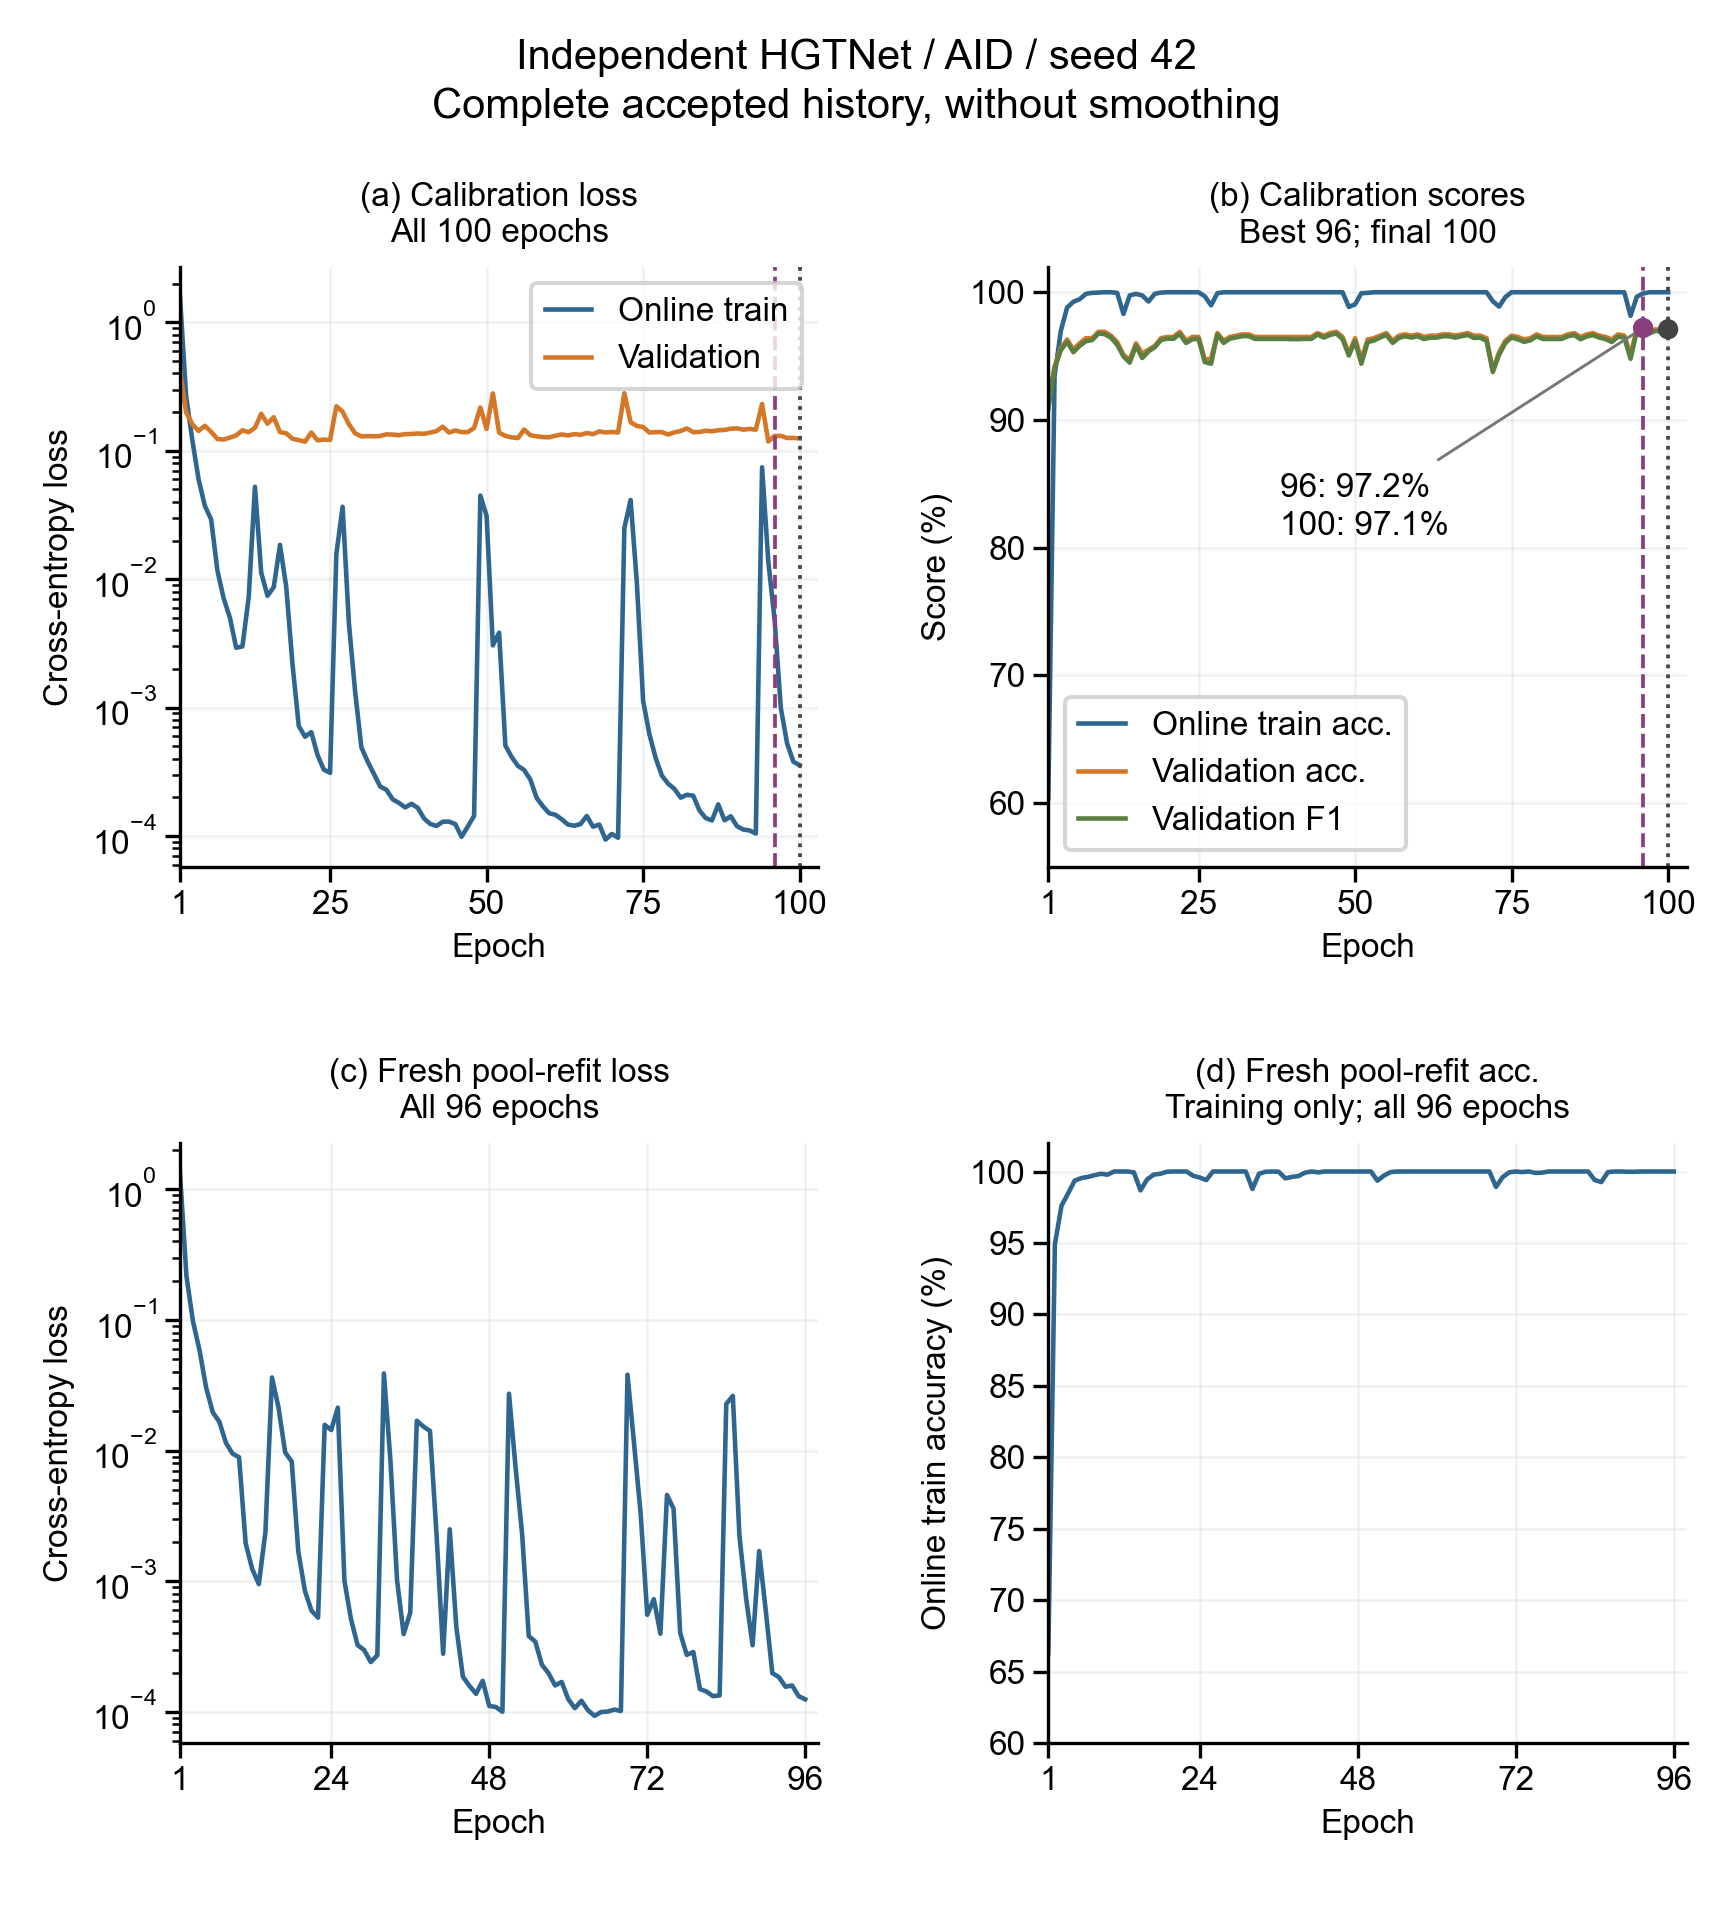
\includegraphics[width=\textwidth]{images/external_aid_20261108/hgtnet_aid_seed42_training_history.png}
 \caption{Complete HGTNet AID seed 42 calibration and fresh-refit histories.
 Calibration runs for 100 epochs and selects epoch 96 using validation only;
 refit starts from the same initial state and runs for 96 epochs on the
 5,000-image pool. Refit training accuracy is not a held-out test metric.}
 \label{fig:external-aid-history}
\end{figure}

The refit is reinitialised from the same initial model state as calibration,
rather than continued from its best checkpoint. An interrupted refit attempt
is resumed from the last committed epoch 75 state. The original partial
updates are retained in the attempt record but excluded from the accepted
trajectory, which finishes with 55,048 optimiser steps. The final checkpoint
is reloaded with zero maximum discrepancy in the recorded reload check,
and the final test transaction completes. This execution evidence supports
the identity of the reported run; it is not an additional training seed.
The reload check was executed on the server, while local verification
recomputes metrics from downloaded records rather than loading the model
binary.

Figure~\ref{fig:external-aid-confusion} shows all 30 classes. The lowest
per-class recalls are Square 143/165 (86.67\%), Center 113/130 (86.92\%),
Resort 129/145 (88.97\%) and School 135/150 (90.00\%). Two largest
bidirectional confusions tie at 12 errors each: Center/Square contributes
6 in each direction, while Park/Resort contributes 4 Park-to-Resort and
8 Resort-to-Park errors. These counts describe the retained test errors.
Without a controlled module intervention or image-level explanatory
evidence, they do not identify graph propagation or a particular visual
structure as the cause.

\begin{figure}[tbp]
 \centering
 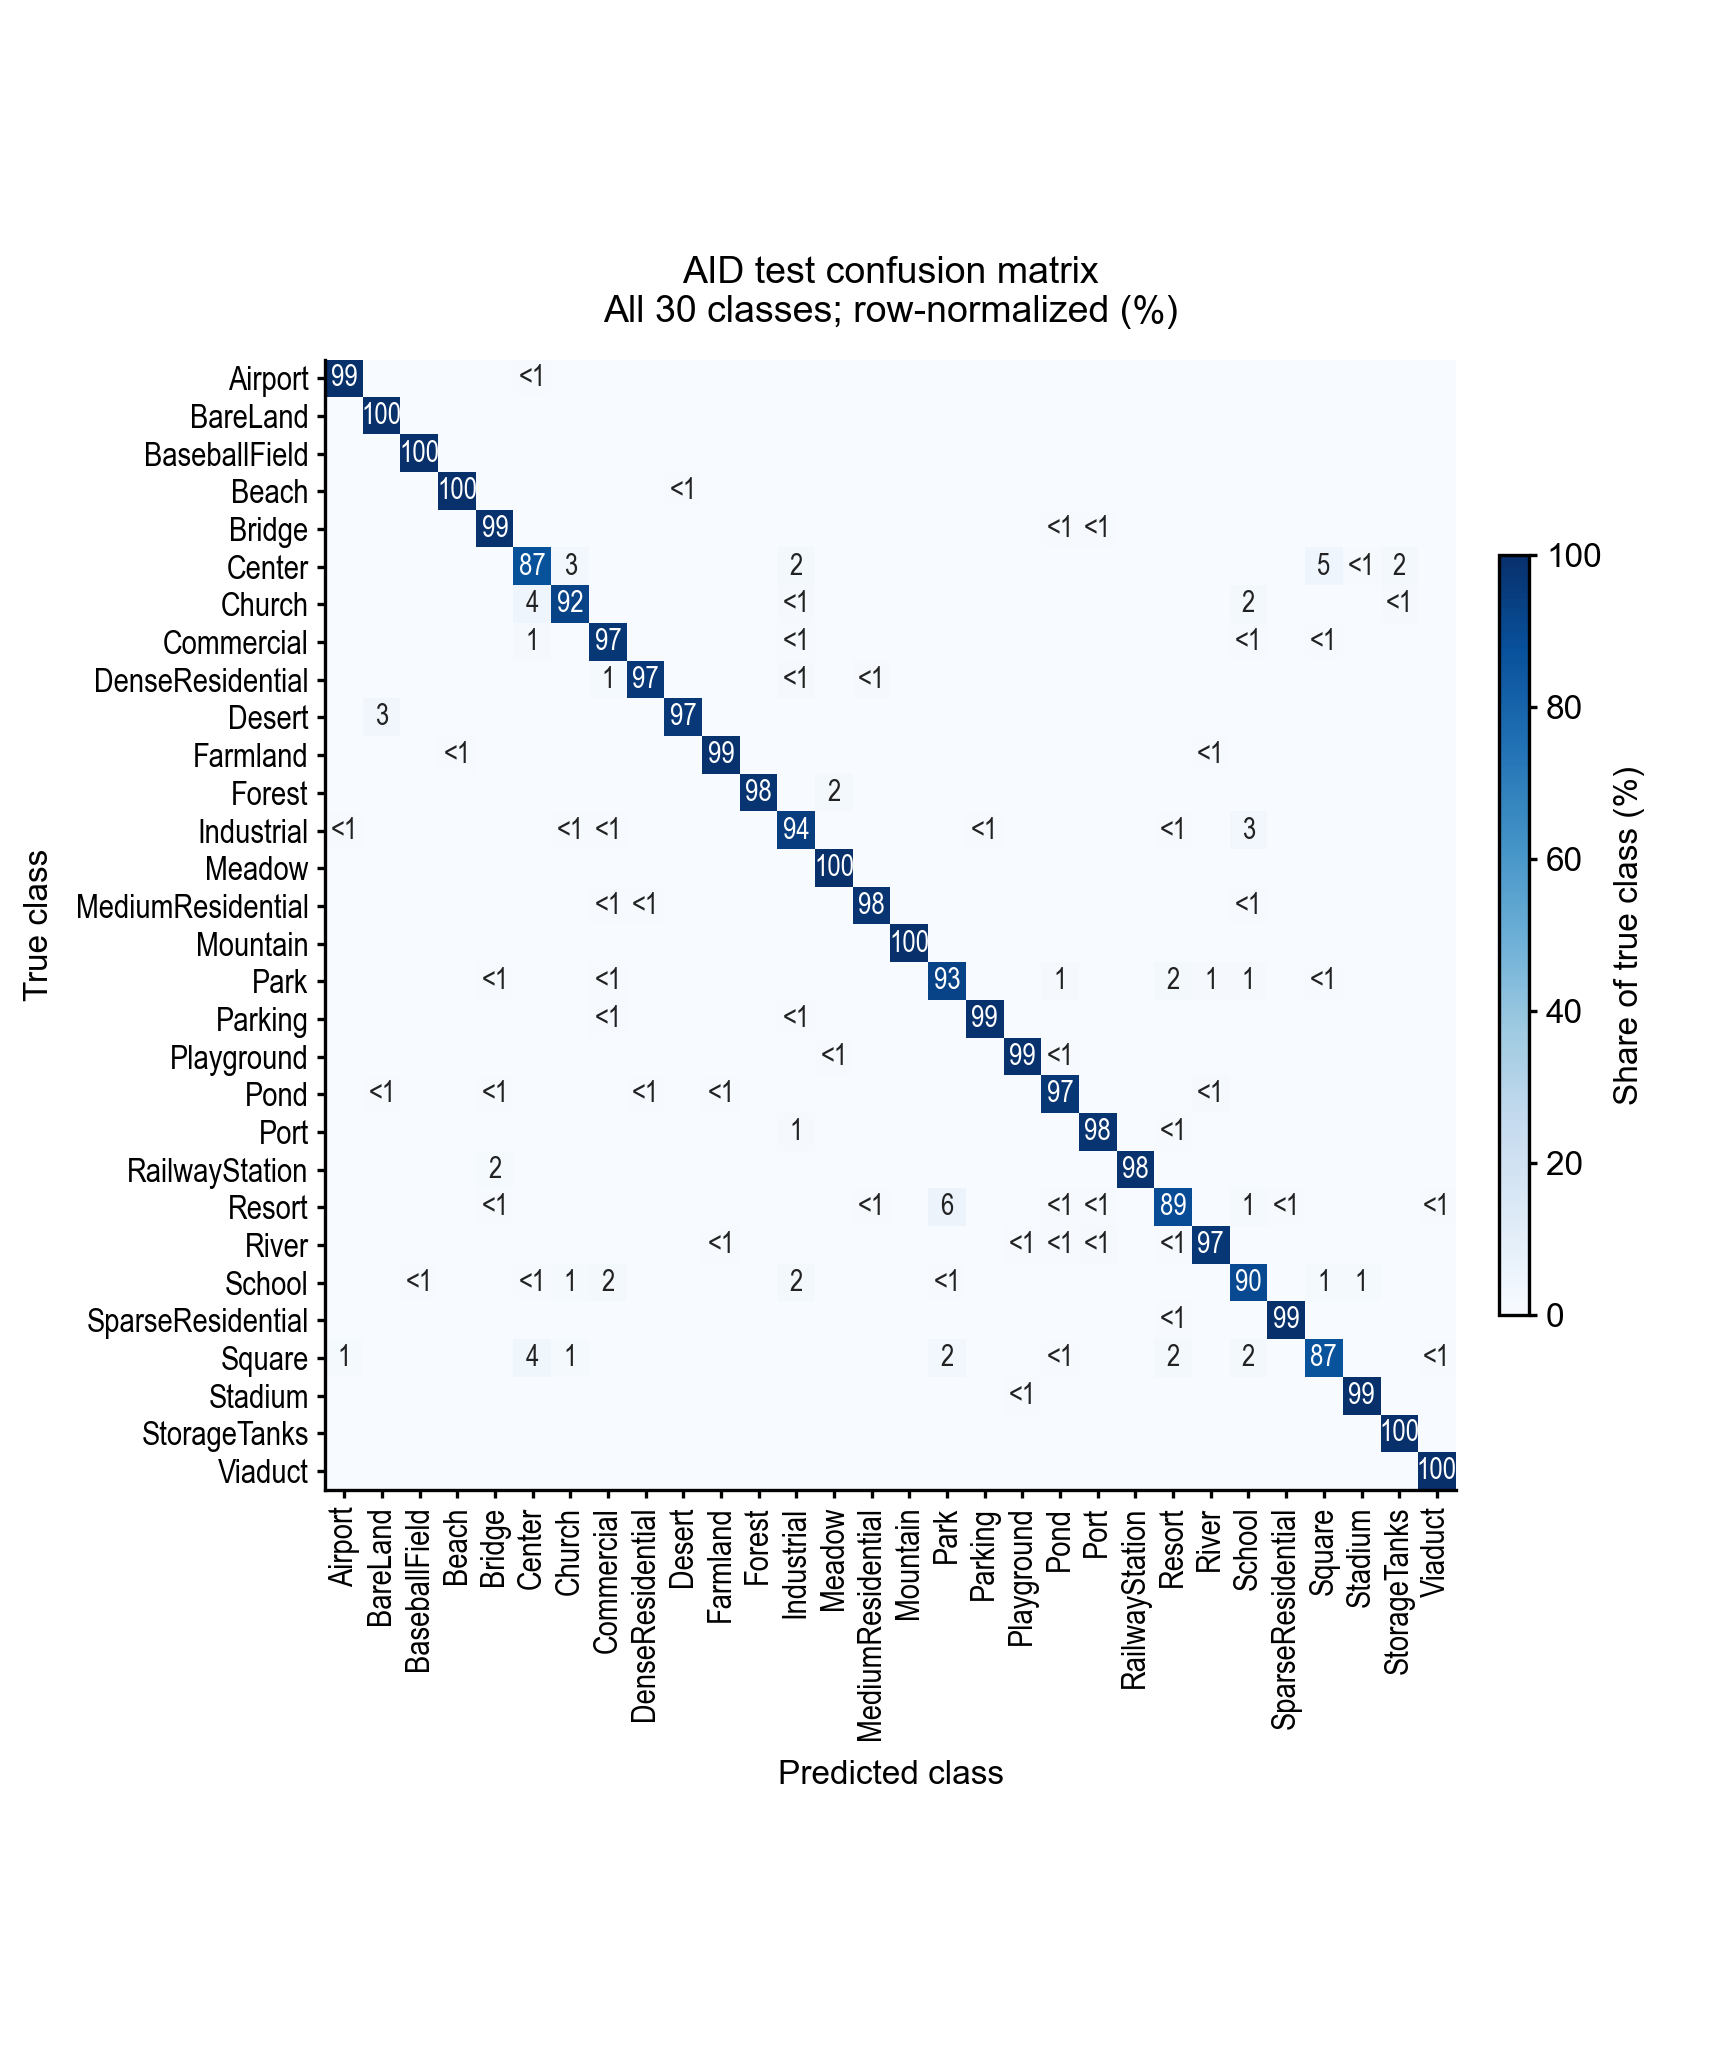
\includegraphics[width=\textwidth]{images/external_aid_20261108/hgtnet_aid_seed42_confusion_matrix.png}
 \caption{HGTNet AID seed 42 confusion matrix for all 5,000 test images.
 Rows are true classes and columns are predictions; each row is normalised
 by its class support. All 30 classes are retained, including classes with
 no observed errors. Colours use unrounded row percentages. Nonzero labels are rounded to
 whole percentages; values below 1\% are shown as $<1$. Exact counts are
 retained in the accompanying records.}
 \label{fig:external-aid-confusion}
\end{figure}

\section{Complexity and remaining comparison requirements}

The full neural parameter count is 31,375,385 for fixed GAViT on AID and
74,612,163 for the independent HGTNet. On NWPU-RESISC45 the corresponding
counts are 31,386,920 and 74,619,858. Fixed GAViT therefore uses approximately
57.95\% fewer parameters on AID and 57.94\% fewer on NWPU, while the OA
point estimates are close in these two seed 42 comparisons. This is a
statement about parameter counts and observed scores, rather than proof
that its extra graph computation is worthwhile relative to Swin-T.
Relative to the 27,543,960-parameter AID Swin-T baseline, fixed GAViT adds
approximately 13.91\% parameters. Its smaller size relative to HGTNet
therefore does not remove the need to justify its extra cost over its
own shared backbone.

The internal seed 42 runs use an RTX 2080 Ti, the DFAGCN NWPU run an RTX 3080,
and the HGTNet NWPU run an RTX 3090. The recovered HGTNet AID result resumes
on an RTX 3060. Its resumed attempt takes 4,986.5883 seconds and records
4.406GiB peak allocated and 4.820GiB peak reserved CUDA memory. These
measurements cover that invocation, including its diagnostics and reload,
rather than the whole experiment or inference alone. Full experiment cost
and peak memory across attempts remain unavailable. Device, timing scope,
preprocessing and training-budget differences prevent a same-device speed
or cost claim from these records.

The supported observation is that the independent HGTNet and fixed GAViT
have close accuracy point estimates on both held-out datasets for seed 42,
with substantially different parameter counts and training recipes.
The independent DFAGCN recipe is lower on NWPU in this run. Neither
observation establishes a stable complete-method ranking, a causal benefit
of a graph component, or equivalence to author-reported results. A final
external main comparison still requires an explicitly unified protocol,
multiple completed training seeds with means and sample standard deviations,
and comparable efficiency measurements. The complete internal results,
architecture ablations and integrated discussion also remain to be added
to this partial thesis draft.
